\section{Intergrated Circuits}

An Intergrated Circuit (IC) is a micro chip that can function as an amplifier, oscillator, timer,
microprocessor, or computer memory.
IC can hold anywhere from hundreds to millions of transistors, resistors and capacitors.
Embedded system is a combination of computer hardware and software designed for functions
within a larger system or for a specific function.


\textbf{Abstraction} when designing a digital system is useful for understanding the system.


\subsection{Moores law}

Moores law states that the number of transistors on a microchip doubles every two years.
This correlates to the transistor size halving every two years.


\section{VHDL}
Very High Speed Integrated Circuit Hardware Description Language.
It is a programming language that has been designed and optimized for describing
the behavior of digital systems.

\subsection{VHDL Syntax}

VHDL is not case sensitive, but it is a good practice to use upper case for keywords and lower case for everything else.
VHDL describes hardware and so instructions are executed in a concurrent manner, meaning that all instructions are executed at once.


Comments are written with two hyphens (- -).


\textbf{if, case and loop statements}

Every if statement has a corresponding then component and each if statement is terminated with an end if;
If an else if statement is needed then it can be written as elsif. Before
each if statement a process statement must be written. The process
statement includes the sensitivity list which is a list of signals that the process is sensitive to.
Once one of the signals in the sensitivity list changes value the process is executed.

\begin{verbatim}
process (sel, I)
begin
  if (sel == "00") then
    a <= 'I';
    b <= '0';
    c <= '0';
    d <= '0';
      
  elsif (sel == "01") then
    a <= '0';
    b <= 'I';
    c <= '0';
    d <= '0';
  elsif (sel == "10") then
    a <= '0';
    b <= '0';
    c <= 'I';
    d <= '0';
  else
    a <= '0';
    b <= '0';
    c <= '0';
    d <= 'I';
  end if;
end process;
\end{verbatim}


Each case statement is terminated with end case; Each loop statement has a corresponding end loop;

\begin{verbatim}
case (expression) is
  when choices =>
    <sequential statements>
  when choices =>
    <sequential statements>
  when others =>
    <sequential statements>
end case;
\end{verbatim}


\textbf{Signal and variable assignments}

Among the most frequently used object types there is the signal object type, the variable object type,
and the constant object type. The signal type is the software representation of a wire in the digital system.
The variable type is used to store local information.
The constant type is used to store constant information.

Signals can be used inside or outside processes. They take the value depend on if the signal is used
in combinational or sequential code.
In combinational code, signals immediately take the value of their assignment. In sequential code,
signals do not immdeiately take the value of their assignment.

Signals are declared at the top of the architecture body, just before the keyword begin.
Variables must be declared inside the process construct but before the begin and are local.
Thus, variables can only be used inside processes.

Assigning a value to a signal is done using the signal assignment operator $<=$.
$$C <= not(A);$$
Assigning a value to a variable is done using the variable assignment operator $:=$.
$$ B := A;$$

A variable changes its value immediately after the variable assignment is executed. Instead a signal
changes its value "some time" after the signal assignment expression is evaluated.

\begin{center}
	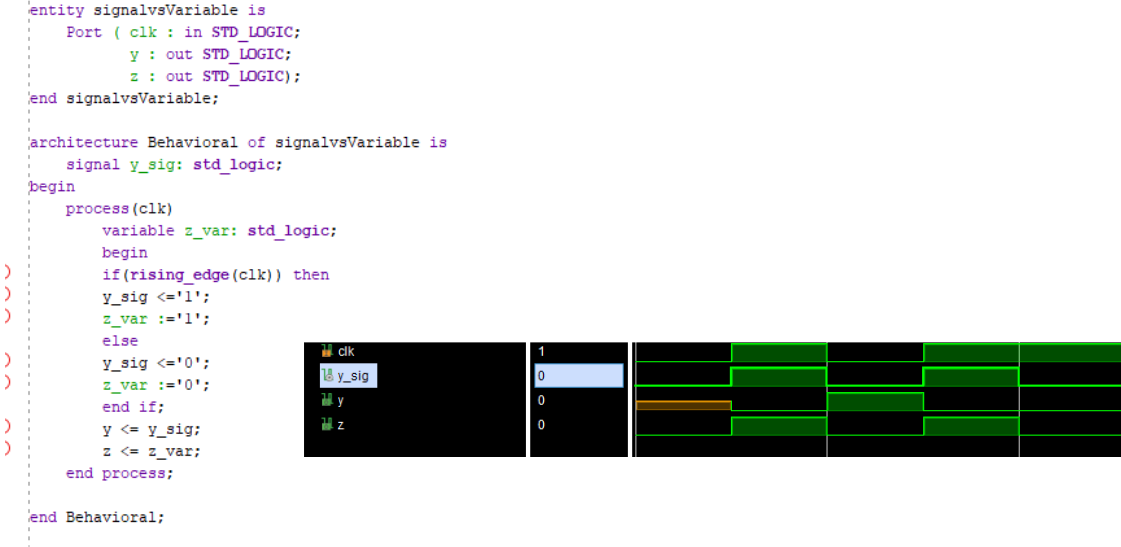
\includegraphics[width=\textwidth]{images/signal_variable.png}
\end{center}


\subsection{VHDL Design Units}


\textbf{STD LOGIC}

\begin{center}
	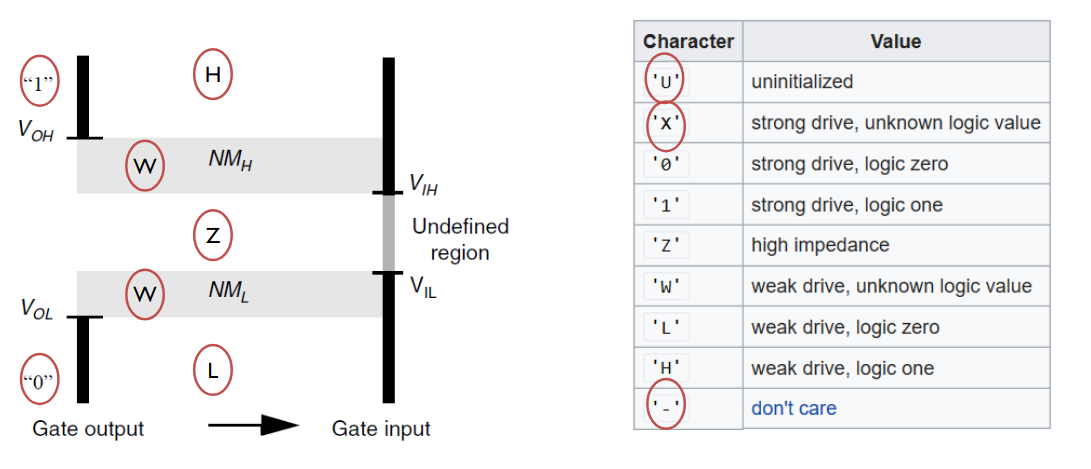
\includegraphics[width = 0.7\textwidth]{images/stdlogic.png}
\end{center}

The noise margins indicate how much noise can be added to the logic level
and still have the logic level recognized as the same.


\textbf{Entity}

The entity describes how the unit interfaces with the outside world.
The entity lists the various inputs and outputs of the underlying system.

\begin{center}
	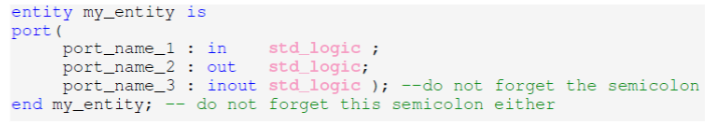
\includegraphics[width=0.8\textwidth]{images/entity.png}
\end{center}

\textbf{Architecture}

Describes what the circuit actually does. It describes the internal
implementation of the associated entity. An architecture can be written by means of three modeling
techniques plus any combination of these three: dataflow, behavioral, and structura plus any combination of these three.


\textbf{Complex logig circuit}

\begin{center}
	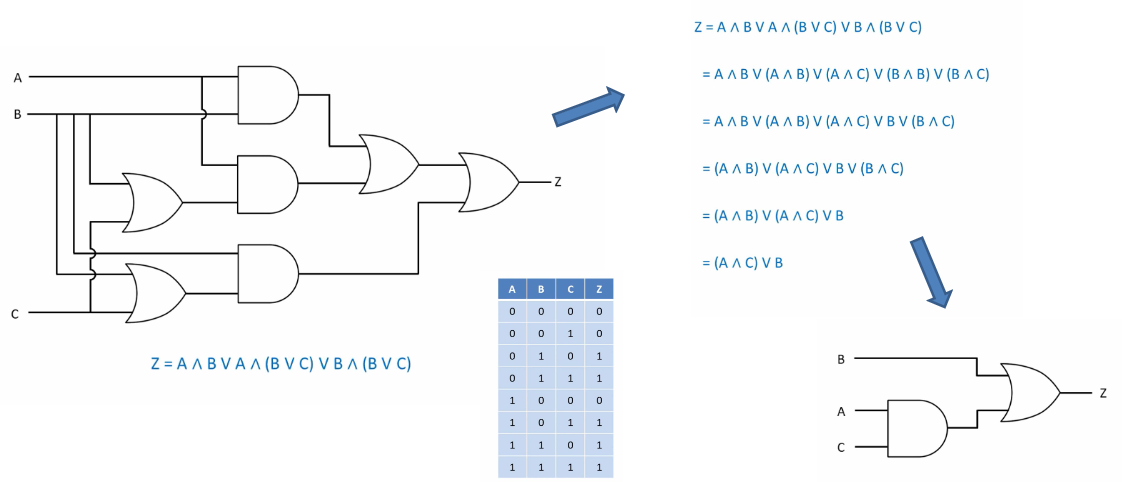
\includegraphics[width=\textwidth]{images/complexLogic.png}
\end{center}


\textbf{Laws of Boolean Algebra}

A $+$ corresponds to an OR gate. An $\cdot$ corresponds to an AND gate.
And a $'$ corresponds to a NOT gate.

In digital electronics, Boolean Algebra is used to simplify the
design of complex circuits.


\textbf{Karnaugh map (K-map)}

A method of circuit optimization. Aims to reduce logic functions
more quickly and easily compared to Boolean algebra.

\begin{center}
	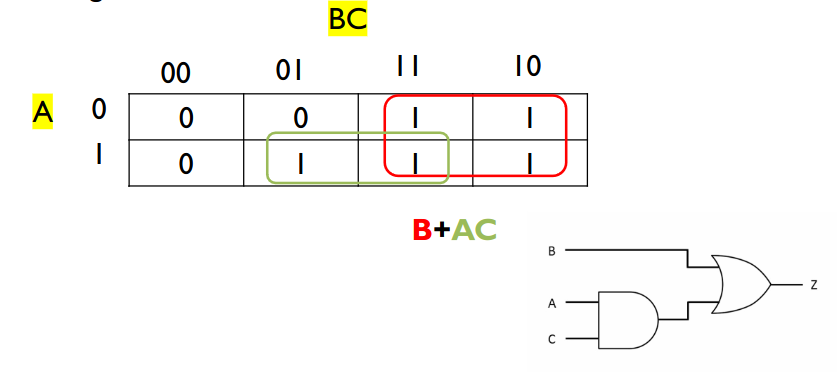
\includegraphics[width=0.8\textwidth]{images/kmap.png}
\end{center}


\textbf{Combinational circuits}

It is defined as the time independent circuits which do not depend upon previous
inputs to generate any output.
e.g. Encoder, Decoder, Multiplexer, Demultiplexer etc.

\textbf{Sequential circuits}

Dependent on clock cycles and depends on present as well as past inputs to generate any output.
e.g. Flip-flops, Counters, Registers etc.


\textbf{Concurrent Statements}
CHDL has the ability to execute a virtually unlimited number of statements at the same time and in a concurrent manner. The key thing to remember is that we are
designing hardware.

\textbf{Conditional Signal Assignment when}

The term conditional assignment is used to describe statements that
have only one target but can have more than one associated expression
assigned to the target.

The individual conditions are evaluated sequentially
in the conditional signal assignment statement until the first
condition evaluates as true.

Conditional signal assignment is a concurrent statement that assigns a
value to a signal based on the value of a condition. The syntax is:

\begin{verbatim}
  <target> <= <expression> when <condition> else 
          <expression> when <condition> else 
          <expression>;
\end{verbatim}

\textbf{Selected Signal Assignment with select}

Selected signal assignments only have one assignment operator. Selected signal assignment
differs from conditional assignment statements in that assignments are based upon the evaluation
of one expression. The syntax is:

\begin{verbatim}
  with <choose_expression> select
    <target> <= <expression> when <choices>,
                <expression> when <choices>
                <expression> when others;
\end{verbatim}

The general form of the selected signal assignment statement is similar to switch statements
as seen in algorithmic programming languages such as C.

\textbf{Process Statements}

The process statement is a stement which contains a certain number of instructions that, when the process statement
is executed, are executed sequentially. In other words the process statement is a tool that can be used
for executing a certain number of instructions in a sequential manner.

The process statement is in itself a concurrent statement.

\textbf{Multiplexer}

The function of a multiplexer is to select one of the inputs
and connect it to the output.

A general multiplexer has n data inputs, one output, and m select inputs.
The number of select inputs determines the number of data inputs.
The number of data inputs is 2 to the power of the number of select inputs.


\begin{center}
	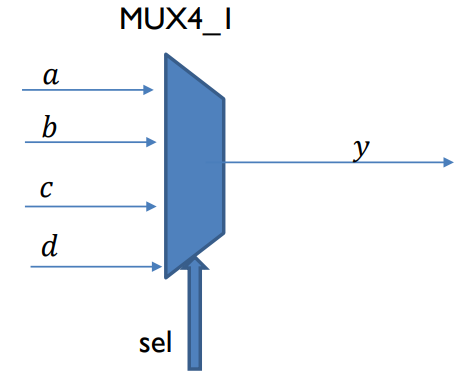
\includegraphics[width=0.3\textwidth]{images/mux.png}
\end{center}


\textbf{Demultiplexer}

It selects one ouput from the multiple output line and feteches the single input through
the selection line.


\begin{center}
	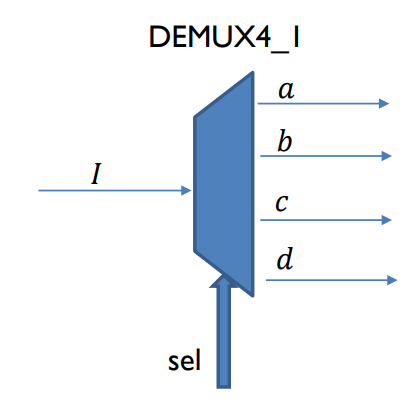
\includegraphics[width=0.2\textwidth]{images/demux.png}
\end{center}


\textbf{Encoders}

Encoders are used to encode data into a coded form and decoders
are used to convert it back into its original form. An encoder that has
$2^n$ input lines and n output lines is called an $n-to-2^n$ encoder.
It is assumed that only one input has a value of 1 at any given time.
It is used to minimize the number of input lines.

Priority encders are a modified version of an encoder. It gives a priority
to an input signal and provides an output based on that priority.

Example of a 4-to-2 priority encoder:

\begin{verbatim}
entity Priority_Encoder is
  port (D: in std_logic_vector(3 downto 0);
        Y: out std_logic_vector(1 downto 0));
end Priority_Encoder;

architecture Behavioral of Priority_Encoder is

begin
  process (D)
  begin
    if (D(3) = '1') then
      Y <= "11";
    elsif (D(2) = '1') then
      Y <= "10";
    elsif (D(1) = '1') then
      Y <= "01";
    elsif (D(0) = '1') then
      Y <= "00";
    else
      Y <= "---";
    end if;
  end process;
end Behavioral;
\end{verbatim}

\textbf{Decoders}

Decoders are used to decode data that has been encoded using a binary encoder.
An n-bit code can represent $2^n$ different values.
An encoder can be used with enable inputs. The enable inputs are used to enable or disable the decoder.


\textbf{Latches}

Level sensitive memory cell that is transparent to signals passing from
the D input to Q output when enabled. It holds the value of D on Q at the
time when it becomes disabled.

Latches with a clear input. The clear input means that when the clear signal
goes to 1 the output is set to 0.
The clear input is essentially the same as a reset signal.


\textbf{D-type Flip-flops}

Is an edge triggered memory device that transfers a signal's value on its
D input to its Q output, when an active edge transition occurs on its clock input.
The output value is held until the next active edge transition occurs.

Rising edge is preferred. Using an implemented function called rising\_edge(clk)
is more robust to noise compared to using clk'event and clk = '1'.

If you want to use flip-flops with reset it is good practice to use asynchronous reset.
An example of asynchronous reset is shown below on the left, and a syncrhonous reset is shown on the right.

\begin{center}
	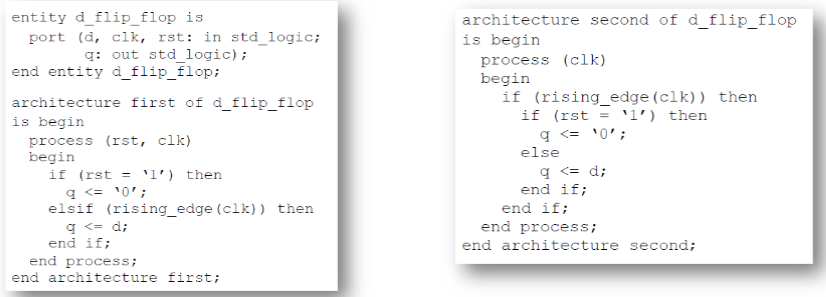
\includegraphics[width=\textwidth]{images/ff_reset.png}
\end{center}



\textbf{Registers}

A parallel register is simply a bank of D-type flip-flops. Its implementation
has the same structure as for one flip-flop but with extended inputs and outputs.


\textbf{Shift registers}

Registers with added features that enable them to shift their contents in either directions.

\begin{center}
	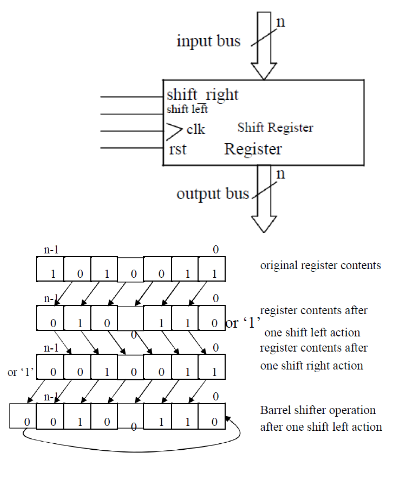
\includegraphics[width=0.6\textwidth]{images/shiftRegister.png}
\end{center}


\textbf{Keypad Encoder}

A device that acts as the link between a keypad and a digital device.
Its primary function is to provide a digital output equal to the
key that is pressed on the keypad.


\textbf{Comparators}

Compares two or more inputs using one, or a number of different comparisons.
When the given relationship(s) is true, an output signal is given
logic 1, otherwise the output signal is given logic 0.

Only two data objects can be compared at once.
Statements like... if (a $=$ b $=$ c) then... are not allowed in VHDL.

Comparators are only modeled using the if statement with an else
clause and no else-if clauses.

Remember that std\_logic\_vector does not indicate a value of the bus.
To compare two buses, unsigned or signes types must be used
for comparision.

\textbf{PWM}

PWM shows how much time the signal is high in an analog fashion.
Duty cycle is used to describe how much of the time
that the signal is on.

\begin{center}
	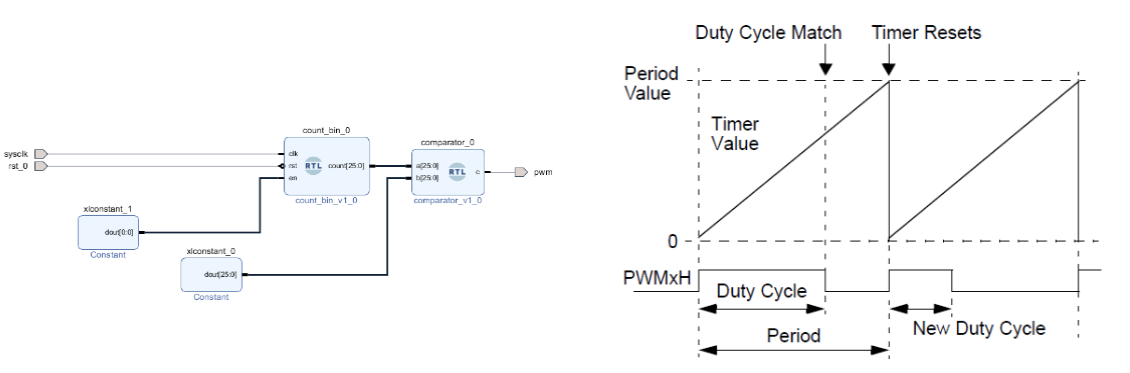
\includegraphics[width=\textwidth]{images/pwm.png}
\end{center}


Calculating how many counter bits that are needed to generate
a PWM signal that has a 1Hz frequency out of a 125MHz clock signal.

$$ n = log_2(125*10^6)$$

\textbf{Adders}

\begin{center}
	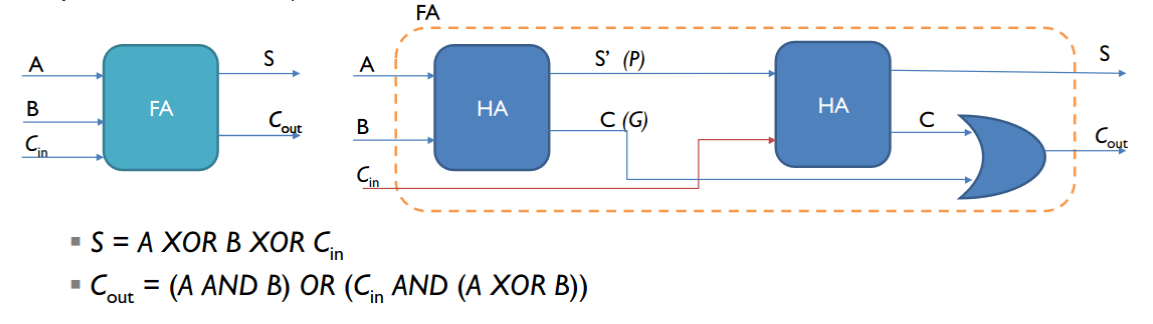
\includegraphics[width=\textwidth]{images/FA.png}
\end{center}

\textbf{Ripple carry adder}

An iterative array to perform binary addition, full adders are chained
together.

\begin{center}
	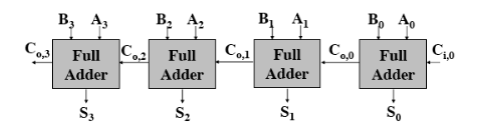
\includegraphics[width=0.6\textwidth]{images/rippleCarry.png}
\end{center}

\textbf{Carry look-ahead adder}

A hierarchical adder that is used to improve performance
because it is faster than the ripple carry adder, but it takes
more resources.

Propagation and Generate.
Propagate means that if there is a carry input, then it is
an XOR operation between the two inputs that decides if
there will be a carry output.

P = A XOR B. The same as sum for a half adder.

G = A AND B. The same as a carry for a half adder.

P and G can be calculated in advance since none of them
depends on the carry bit (Cin).

\begin{center}
	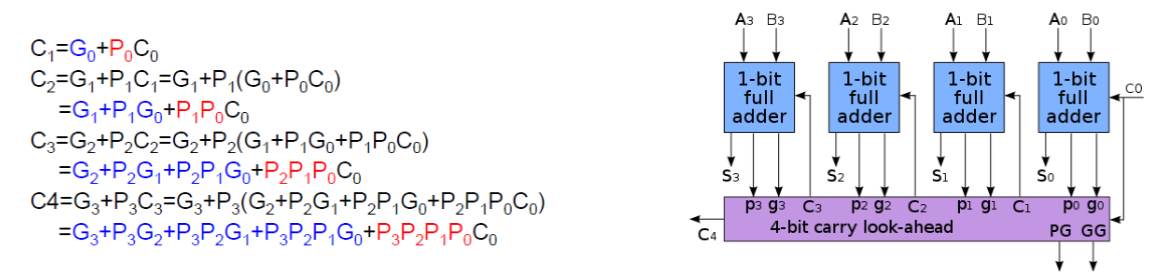
\includegraphics[width=\textwidth]{images/lookAhead.png}
\end{center}


\textbf{Subtractors}

Subtraction can be done by adding 2's complement of the number.
Example for A-B:

\begin{center}
	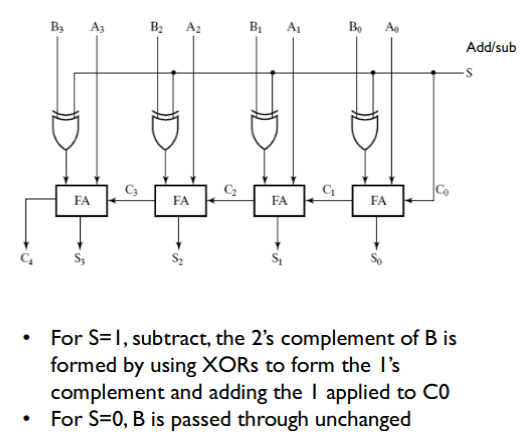
\includegraphics[width=0.6\textwidth]{images/subtract.png}
\end{center}


\textbf{Multiplication}

It can be implemented by a shift register as wide as the product
and an accumulator for the partial and final product.

\begin{center}
	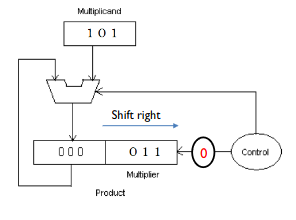
\includegraphics[width=0.6\textwidth]{images/multiplicationBlock.png}
\end{center}

\begin{center}
	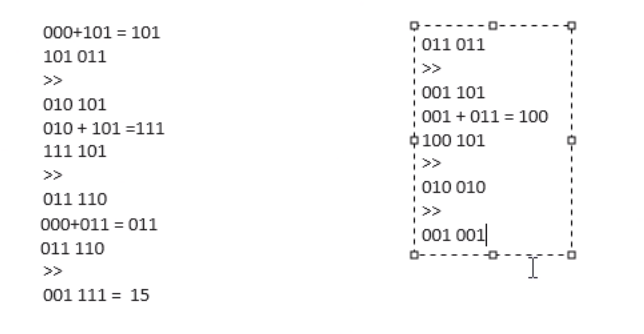
\includegraphics[width=0.6\textwidth]{images/multiplication.png}
\end{center}




\textbf{Dividers}

Division is the most complex of the four basic arithmetic operations.
Hardware solutions are correspondingly larger and more complex
than the solutions for other operations, it is best to minimize the
number of divisions in any algorithm.

Division can be done using a clock divider, by subtraction
and by multiplication.

$$ A \cdot \frac{1}{B} = A \cdot (2^n/B)2^n$$

$$ \frac{10}{4} = 10 \cdot \frac{2^2/4}{2^2} = 10 \frac{1}{2^2} = 10.10$$




\subsection{Standard models in VHDL Architecture}


\textbf{Data-flow style architecture (RTL)}

Describes how data is transformed as it is passed from register to register.
The transformation of data is performed by the combinational logic
that exists between the registers. For example, logic gates, multiplexers,
flip flops etc.


\textbf{Behavioral style architecture}

It provides no details as to how the design is implemented in actual hardware.
The behavioral style models how the circuit outputs will react to the circuit inputs.
Whereas in data-flow modeling you somewhat need to have a feel for the underlying logic in the circuit.
In other words, data-flow modeling describes how the circuit should look in terms of logic gates
whereas behavioral modeling describes how the circuit should behave.

\textbf{Structural}

Describes the interconnection of components within an architecture.
For example block design.

\textbf{Hybrid style}

A combination of the previous design styles.


\subsection{Simulation vs Synthesis}

Simulation-only operations for error messages or reading files that
can be simulated but not synthesized.

Constructs such as for loops, while loops, etc. are either
un-synthesizable or (worse) synthesize poorly.

You need procedural code for testbench and only for testbench.
Examples: AND gate is synthesizable but AND gate with 5ns wait is not.
Printf is not synthesizable.

Use synthesizable code to describe the function of units that will be
built into hardware. Use non-synthesizable code to create a testbench
that checks to see if your synthesizable code does what you want.

\textbf{Synthesis} is a process of converting high level
FPGA logic design into gates.


